\documentclass[12pt, a4paper]{article}
\usepackage[utf8]{inputenc}
\usepackage[spanish]{babel}
\usepackage{amsmath, amssymb}
\usepackage{graphicx}
\usepackage[margin=2.5cm]{geometry}

\title{Trabajo Practico Numero 1}
\author{Minería de Datos}
\date{\today}

\begin{document}

\maketitle

\section{Medidas descriptivas (media, cuartiles, etc.)}

Para una variable \(x_1,\dots,x_n\):

\begin{itemize}
    \item \textbf{Media:} \(\bar{x} = \frac{1}{n}\sum_{i=1}^{n} x_i\)
    \item \textbf{Mediana:}
    \begin{itemize}
        \item Ordenar los datos.
        \item Si \(n\) es impar: posición \(\frac{n+1}{2}\)
        \item Si \(n\) es par: promedio entre las posiciones \(\frac{n}{2}\) y \(\frac{n}{2}+1\)
    \end{itemize}
    \item \textbf{Q1 y Q3:} se calculan sobre datos ordenados (\textit{aclarar el criterio que usan, porque hay varios}).
    \item \textbf{Rango Intercuartílico (RI):} \(RI = Q3 - Q1\)
\end{itemize}

\textbf{En el informe:}
\begin{itemize}
    \item Poner una tabla con valores ordenados y posiciones.
    \item Marcar qué elementos corresponden a Q1, mediana, Q3.
\end{itemize}

\hrule\vspace{0.5cm}

\section{Discretización por frecuencia}

Los cortes numéricos calculados son: \(1.0\), \(4.5\) y \(22.0\).

\vspace{0.5cm}
\begin{center}
\renewcommand{\arraystretch}{1.5}
\begin{tabular}{|l|c|c|}
    \hline
     & \textbf{Baja} & \textbf{Alta} \\
    \hline
    \textbf{Intervalos} & \([1.0, 4.5]\) & \((4.5, 22.0]\) \\
    \hline
    \textbf{Valores} & 5 & 5 \\
    \hline
\end{tabular}
\end{center}
\vspace{0.5cm}

\begin{figure}[htbp]
    \centering
    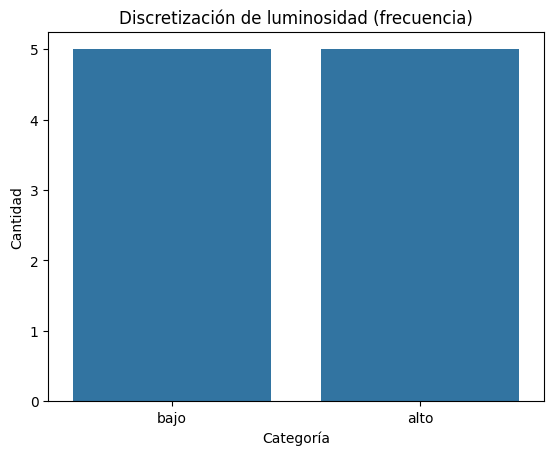
\includegraphics[width=0.75\textwidth]{imagenes/discretizacion_luminosidad_frecuencia.png}
    \caption{Gráfico de cantidad de estrellas por categoría de luminosidad.}
    \label{fig:freq_lum}
\end{figure}

\hrule\vspace{0.5cm}

\section{Discretización por rango }

Los cortes numéricos calculados son: \(0.979\), \(11.5\) y \(22.0\).

\vspace{0.5cm}
\begin{center}
\renewcommand{\arraystretch}{1.5}
\begin{tabular}{|l|c|c|}
    \hline
     & \textbf{Baja} & \textbf{Alta} \\
    \hline
    \textbf{Intervalos} & \((0.979, 11.5]\) & \((11.5, 22.0]\) \\
    \hline
    \textbf{Valores} & 8 & 2 \\
    \hline
\end{tabular}
\end{center}
\vspace{0.5cm}

\begin{figure}[htbp]
    \centering
    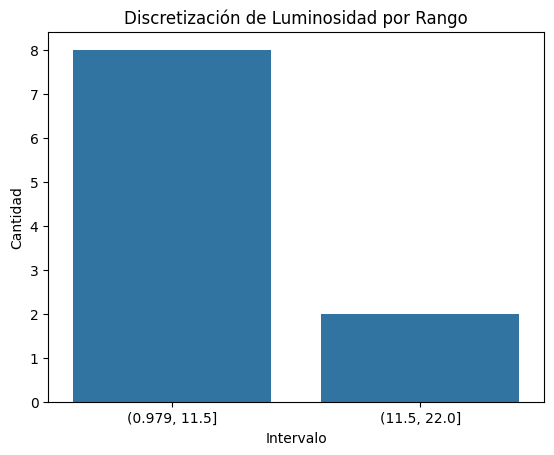
\includegraphics[width=0.75\textwidth]{imagenes/Discretizacion_de_luminosidad_por_rango.png}
    \caption{Gráfico de cantidad de estrellas por rango de luminosidad.}
    \label{fig:rango_lum}
\end{figure}

\hrule\vspace{0.5cm}

\section{Correlación lineal (Pearson) }

Al calcular la correlación lineal de Pearson entre la Luminosidad y la Temperatura, se obtuvieron los siguientes resultados:

\vspace{0.5cm}
\begin{center}
\renewcommand{\arraystretch}{1.5}
\begin{tabular}{|l|c|}
    \hline
    \textbf{Atributo} & \textbf{Valor} \\
    \hline
    \textbf{Correlación Lineal} & \(0.5878\) \\
    \hline
    \textbf{Intensidad} & Débil \\
    \hline
    \textbf{Tipo} & Positiva \\
    \hline
\end{tabular}
\end{center}
\vspace{0.5cm}

\begin{figure}[htbp]
    \centering
    % En caso de haber guardado la imagen, descomentar y ajustar el nombre:
    % \includegraphics[width=0.7\textwidth]{imagenes/correlacion_luminosidad_temperatura.png}
    \caption{Diagrama de dispersión de Luminosidad vs Temperatura.}
    \label{fig:corr}
\end{figure}

\hrule\vspace{0.5cm}

\section{Diagrama de Caja de Tukey ``a mano''}

Se calculó el diagrama de caja de Tukey para la variable \textbf{Luminosidad}. Los resultados se muestran en la tabla a continuación:

\vspace{0.5cm}
\begin{center}
\renewcommand{\arraystretch}{1.5}
\begin{tabular}{|l|c|}
    \hline
    \textbf{Parámetro} & \textbf{Valor} \\
    \hline
    \textbf{Mediana (Q2)} & \(4.5000\) \\
    \hline
    \textbf{Q1 (Cuartil 1)} & \(3.0000\) \\
    \hline
    \textbf{Q3 (Cuartil 3)} & \(5.7500\) \\
    \hline
    \textbf{RI (Rango Intercuartil)} & \(2.7500\) \\
    \hline
    \textbf{Bigote superior} & \(6\) \\
    \hline
    \textbf{Bigote inferior} & \(1\) \\
    \hline
    \textbf{Intervalo de valores atípicos leves} & \([-1.1250, 9.8750]\) \\
    \hline
    \textbf{Valores atípicos leves} & \(16, 22\) \\
    \hline
    \textbf{Intervalo de valores atípicos extremos} & \([-5.2500, 14.0000]\) \\
    \hline
    \textbf{Valores atípicos extremos} & \(16, 22\) \\
    \hline
\end{tabular}
\end{center}
\vspace{0.5cm}

\begin{figure}[htbp]
    \centering
    % En caso de haber guardado la imagen, descomentar y ajustar el nombre:
    % \includegraphics[width=0.7\textwidth]{imagenes/diagrama_caja_tukey.png}
    \caption{Diagrama de Caja de Tukey para Luminosidad.}
    \label{fig:tukey}
\end{figure}

\end{document}